\documentclass{llncs}
\usepackage{graphicx}
\usepackage{booktabs}
\begin{document}
\title{
\includegraphics[scale=0.6]{university-of-amsterdam.png}\\{Do countries practice what they preach?}}
\subtitle{Assignment 1 - Fundamentals of Data Science}
\author{Emmi Lidman \and Michail Mavrokoukoulakis \and Vaamika Rajsingh\ \and Sem de Regt}
\institute{University of Amsterdam\\
\today}
\maketitle
\newpage
\begin{abstract} ... \keywords{UN General Debate \and SDGs \and NLP} \end{abstract}
\section{Introduction}
Every September, representatives of the UN member states gather in New York for the general debate of the United Nations General Assembly. There, heads of state and senior officials present their government's view on the most pressing of matters in world politics. These statements are delivered annually by nearly every country in the world and they form a unique record of how countries wish to present themselves to the international community. Every general debate has a theme, and the theme of this years 81st session in 2026 is \textit{"Leaving no one behind: acting together for the advancement of peace, sustainable development and human dignity for present and future generations."}.

This years theme is closely linked to Sustainable Development Goal 13 (SGD-13), \textit{"Take urgent action to combat climate change and its impacts"}, which on countries to integrate climate change measures into national policies and strategies, and under the 2015 Paris Agreement nearly all states have made public climate pledges. Trust in these commitments, however, depends on whether words are followed by action. Climate change has become a recurring topic in the General Debate, but it is unclear to what extent the attention a country gives to climate in its speeches reflects its actual emissions and energy transition. In other words, do they practice what they preach?

In this report, we combine the UN General Debate Corpus (UNGDC) \cite{jankin2025words}\cite{baturo2017understanding}, which contains the statements from every General Debate session from 1946 to 2025, with coal, natural gas, and oil rents from the World Bank \cite{worldbank_wdi_coal}\cite{worldbank_wdi_gas}\cite{worldbank_wdi_oil}, as well as two datasets from Our World in Data (OWID): one on countries' energy mixes \cite{owid-energy-mix} and one on fossil-fuel production \cite{owid-fossil-fuel-production}, to address two questions:

\begin{enumerate}
    \item[\textbf{RQ1}] \textit{(Exploratory)} [What is the correlation between the frequency of energy transition related mentions by the world's top fossil-fuel-producing countries in their UN General Debate speeches and their fossil fuel consumption following the 2015 Paris Agreement?]
    \item[\textbf{RQ2}] \textit{(Predictive)} [Does how a country talks about the energy transition — how often, and how cautiously — predict whether its fossil fuel production rises or falls since the Paris Agreement, and is that relationship different for major exporters than for everyone else?
]
\end{enumerate}

\section{Methodology} 
\subsection{UN General Debate Corpus} 

Our base dataset is the United Nations General Debate Corpus, which contains the statements delivered in
the General Debate from Session~1 (1946) to Session~80 (2025). Each statement
is stored as a separate text file whose name encodes the country's ISO-alpha3
code, the session number and the year. Our pre-processing of this corpus is
deliberately light: every step is there because a later step of the analysis
requires it, and we do not apply standard cleaning steps that our method does
not need.

\subsubsection{Loading.}
We read all files into a single table with one row per speech, resulting in
11{,}141 speeches from 200 countries and entities.

\subsubsection{Metadata.}
We added each country's name, region and sub-region from the UN Statistics
Division M49 standard, so that countries can be compared across
regions. We used a left join so that no speech is lost. For 150 speeches no
region was found; these belong to states that no longer exist
(Czechoslovakia, East Germany, South Yemen and Yugoslavia) and to the European
Union, which speaks as an observer. We kept them in the corpus and exclude
them only where a region or country-level indicator is required.

\subsubsection{Text normalisation.}
The speeches were digitised from printed documents, so some words are split
across two lines with a hyphen (e.g.\ ``in-vestment''). Because our method
searches for specific words and phrases, such split words would not be found.
We rejoined 7{,}891 of these words and replaced all tabs, line breaks and
repeated spaces with a single space.

\subsubsection{Steps we deliberately omitted.}
We did not convert the text to lowercase, remove punctuation or remove stop
words, although these are common steps in text analysis. Splitting a speech
into sentences relies on capital letters and full stops, and our phrase
matching already ignores case. More importantly, standard stop-word lists
remove words such as \textit{will}, \textit{may} and \textit{could}. These are
exactly the words that signal commitment or caution, so removing them would
erase what we want to measure. Since our method only counts words and phrases
that we define ourselves, filtering out other words has no benefit.

\subsubsection{Speech length.}
Speeches range from 423 to 22{,}003 words (median 2{,}550). Since a longer
speech naturally contains more mentions of any topic, we recorded the length
of each speech in words, which allows us to express mentions relative to
speech length.

\subsubsection{Validation.}
Finally, we checked that the number of speeches did not change during the
merges, that every combination of country and year appears only once, and
that no speech became empty after cleaning.


\subsection{External datasets}
In addition to the UN General Debate Corpus, we used five external datasets. Three come from the World Bank's World Development Indicators and report oil, coal, and natural gas rents as a percentage of GDP per country per year \cite{worldbank_wdi_oil} \cite{worldbank_wdi_coal}\cite{worldbank_wdi_gas}, which we use as a measure of how economically dependent a country is on fossil fuels. The other two come from Our World in Data (OWID): the share of primary energy consumption that comes from fossil fuels \cite{owid-energy-mix}, and the annual production of coal, oil, and gas (in TWh) per country \cite{owid-fossil-fuel-production}.

\subsubsection{Loading}
All five datasets were loaded from CSV files into pandas DataFrames. The World Bank files required extra handling: each begins with four metadata rows, which we skipped, and stores the data in wide format, with one row per country and one column per year (1960--2025). The OWID files were already in long format, with one row per country-year.

\subsubsection{Cleaning and converting}
To combine the datasets with each other and with the speech data, which is organized per country per year, we converted all of them to the same long format. We reshaped each World Bank file with \texttt{pandas.melt}, keeping only the country name, ISO-3 code, year, and indicator value, and merged the three indicators on country, ISO-3 code, and year, so that each row holds the oil, coal, and gas rents of one country-year. These were also summed into a single total fossil-fuel rents variable.

Both sources also contain aggregate rows, such as ``World'', ``European Union'', or ``Middle East \& North Africa'', which do not correspond to a country that delivers a speech. For the World Bank data, we removed these using the accompanying country metadata file, in which aggregates have no region assigned; for the OWID data, we kept only rows with a valid three-letter ISO-3 code, since OWID assigns aggregates custom codes such as \texttt{OWID\_WRL}. We renamed the OWID columns to match the World Bank data (e.g.\ \texttt{Entity} $\rightarrow$ \texttt{country}, \texttt{Code} $\rightarrow$ \texttt{iso3}) and finally merged all three sources into one country-year panel keyed on ISO-3 code and year, the same identifiers used for the speeches in the corpus.

\subsubsection{Caveats}
The World Bank rent data is only complete up to 2021; values from 2022 onwards are missing due to reporting delays. The OWID datasets cover only 79 (energy mix) and 73 (production) countries, because their underlying source, the Energy Institute's \textit{Statistical Review of World Energy}, only reports on major energy-producing and -consuming countries. Neither caveat substantially limits our analysis: the post-2015 period is largely covered, and the 19 largest fossil-fuel producers, on which our questions focus, are all included in both OWID datasets.

\subsection{Exploratory Data Analysis}
To answer our first research question: What is the correlation between the frequency of energy transition related mentions by the world's top fossil-fuel-producing countries in their UN General Debate speeches and their fossil fuel consumption following the 2015 Paris Agreement? We needed Exploratory data analysis.

\subsubsection{Defining world's top fossil-fuel-producing countries}
To define the world's top fossil-fuel-producing countries after 2015 we explored our external data sets to find which countries produced the most fossil fuels. To find these countries we looked which countries had the highest production of fossil fuels in twh from the OIWD dataset, and which had a high rent of GDP of fossil fuel exports. To define what was a high production of fossil fuels we took the top quartile producers from the OIWD data set which got cut off at 1642.66twh production and which resulted in 19 major fossil fuel producers. 

\begin{figure}[htbp]
    \centering
    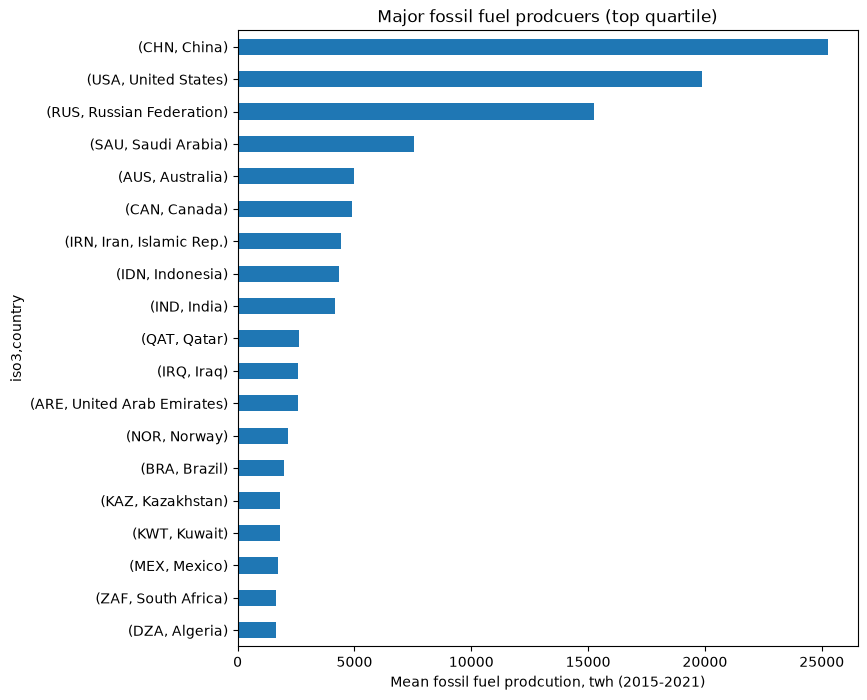
\includegraphics[width=0.8\textwidth]{output.png}
    \caption{world's top fossil-fuel-producing countries after 2015}
    \label{fig:plot}
\end{figure}

To ensure we got the biggest fossil-fuel-producing countries we also intersected it with the biggest exporters of fossil fuels which where determined in a similar fashion. With the rents data we can determine which countries can be seen as the worlds top exporters of fossil fuels here we also took the top quartile exporters which were countries with or more than 1.40\% of GDP which led to 51 major fossil fuel exporters.

\begin{figure}[htbp]
    \centering
    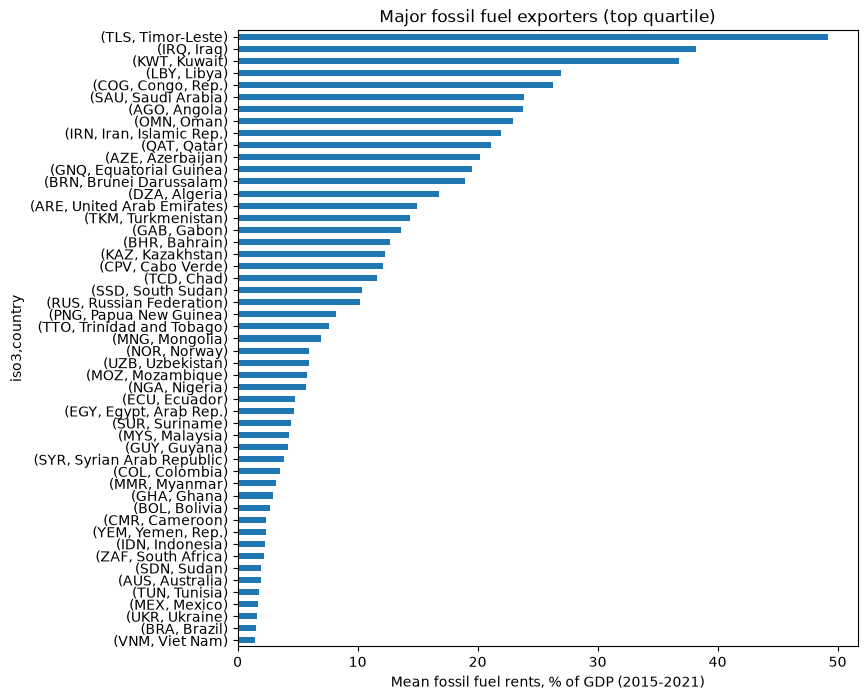
\includegraphics[width=0.8\textwidth]{exporters.png}
    \caption{world's top fossil-fuel-exporting countries after 2015}
    \label{fig:plot}
\end{figure}

When we intersected the two groups we got 15 countries classified as major producers of fossil fuel. These are the countries which are present in both groups and can be seen as the worlds biggest fossil-fuel-producing countries.

\begin{table}[htbp]
    \centering
    \caption{Major fossil fuel producing countries after 2015.}
    \label{tab:major_producers}
    \begin{tabular}{ll}
        \toprule
        ISO3 & Country \\
        \midrule
        ARE & United Arab Emirates \\
        AUS & Australia \\
        BRA & Brazil \\
        DZA & Algeria \\
        IDN & Indonesia \\
        IRN & Iran, Islamic Rep. \\
        IRQ & Iraq \\
        KAZ & Kazakhstan \\
        KWT & Kuwait \\
        MEX & Mexico \\
        NOR & Norway \\
        QAT & Qatar \\
        RUS & Russian Federation \\
        SAU & Saudi Arabia \\
        ZAF & South Africa \\
        \bottomrule
    \end{tabular}
\end{table}

\subsection{Predictive analysis}
To answer the predictive question and therefore asses whether countries rhetoric on the energy transition is reflected in their actual fossil fuel production, three sources were combined: year-over-year change in total fossil fuel production, a classification of major fossil fuel exporting countries as well as two speech-derived measures from the UNGDC corpus which included mention rate (the frequency of energy-transition-related keywords, normalized by speech length) along with net caution (hedging derived from lexicon-and grammar-based detection). Because the transition-rhetoric measures are only meaningfully defined for speeches from 2015, the year of the Paris Agreement, after which such rhetoric becomes common in diplomatic discourse, the analytic sample was restricted to this period. The final merged dataset containing all features and the target yielded 787 country-year observations. 

The target variable, production change, was winsorised at the 1st and 99th percentiles to limit the influence of extreme year-over-year swings, that is countries beginning or creasing production, without discarding observations. Mention rate and net caution were mean-centered and interaction terms with exporter status were included in to test whether the relationship between rhetoric and production differs for major exporters. The data was split chronologically rather than randomly to reflect the time structure of the data and to avoid future information from leaking into training. The training data used the earliest 80\% of the data and the test data used the remaining 20\%. To fit the data an Ordinary Least Squares regression model was used and initial residual diagnostics showed strong non-normality with for instance a skewness of 3.62 and a kurtosis of 31.4. This indicated heteroskedasticity, the spread of errors in the model weren't constant across the values, and the model was therefore refit using heteroskedasticity-consistent (HC3) standard errors. 

\section{Results \& Discussion}
Figure ~\ref{fig:ols_results} reports the coefficient estimates under HC3 standard errors. None of the predictors reached statistical significance at conventional thresholds, exporter status ($\beta = 0.017, p = 0.130$), mention rate ($\beta = 24.08, p = 0.494$), net caution ($\beta = 0.068, p = 0.278$), and their interactions with exporter status (mention rate $\cdot$ exporter and net caution $\cdot$ exporter) were all statistically indistinguishable from zero. The model as a whole was also not significant and explains almost non of the variance in production change ($R^2 = 0.0201$). 

Notably, mention rate initially appeared marginally significant under standard OLS errors ($p = 0.047$), however this did not survive correction for heteroskedasticity once the residual diagnostics indicated that the constant variance assumption was violated. 

On the test set the model achieved an Root Mean Squared Error (RMSE) of 0.1528 and an $R^2$ of 0.0201, indicating it explains only a small fraction of variance beyond the sample mean. Looking at the scores together after HC3 standard errors, there are no findings of evidence that transition-related rhetoric or exporter status predicts following fossil fuel production change in this sample. This may, as discussed above, partly reflect limited statistical power given the heavily zero-inflated mention rate variable with a median of 0, or possibly a genuine disconnect between diplomatic rhetoric and material production. 

\begin{figure}
    \centering
    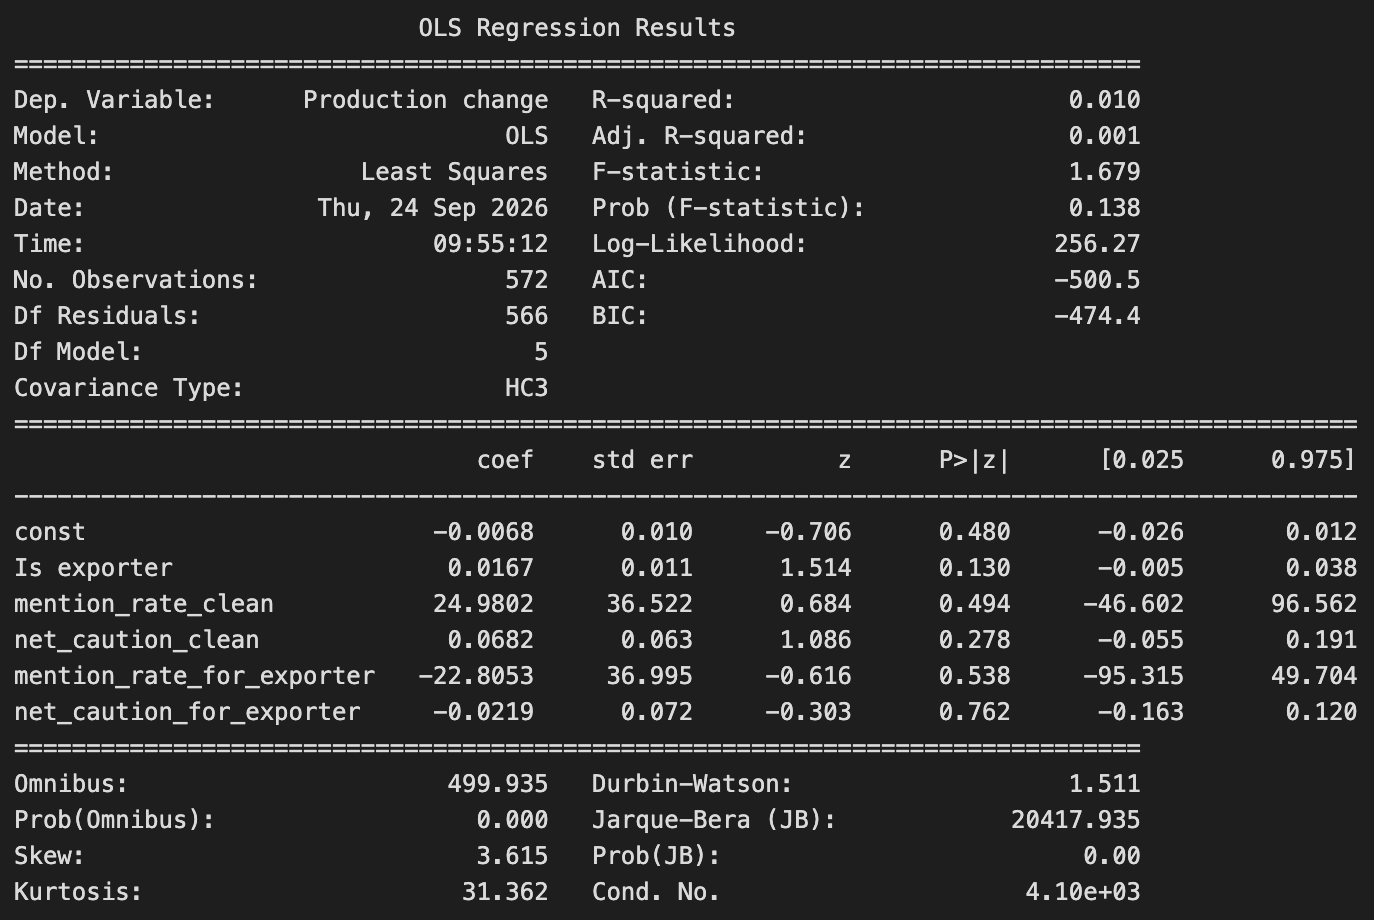
\includegraphics[width=0.5\linewidth]{ols_results.png}
    \caption{OLS Regression results}
    \label{fig:ols_results}
\end{figure}

\section{Conclusion}

\section{References}

\bibliographystyle{splncs04}
\bibliography{references}

\end{document}